\documentclass[10pt]{article}

\usepackage[margin=0.75in]{geometry}
\usepackage{amsmath,amsthm,amssymb}
\usepackage{xcolor}
\usepackage{cancel}
\usepackage{graphicx}
\usepackage{changepage}
\usepackage{circuitikz}
\usepackage{pgfplots}
\usepackage{physics}
\usepackage{hyperref}
\usepackage{siunitx}
\usepackage[breakable]{tcolorbox}
\usepackage[inline]{enumitem}

\theoremstyle{definition}
\newtheorem{problem}{Problem}
\newtheorem{soln}{Solution}

\pgfplotsset{compat=newest}
\usetikzlibrary{lindenmayersystems}
\usetikzlibrary{arrows}
\usetikzlibrary{calc}

\definecolor{incolor}{HTML}{303F9F}
\definecolor{outcolor}{HTML}{D84315}
\definecolor{cellborder}{HTML}{CFCFCF}
\definecolor{cellbackground}{HTML}{F7F7F7}
\newcommand{\eq}{=}
\usetikzlibrary{positioning, fit, calc}
\pgfdeclarelayer{background}  
\pgfsetlayers{background,main}

\makeatletter
\newcommand{\boxspacing}{\kern\kvtcb@left@rule\kern\kvtcb@boxsep}
\makeatother
\newcommand{\prompt}[4]{
    \ttfamily\llap{{\color{#2}[#3]:\hspace{3pt}#4}}\vspace{-\baselineskip}
}

\newcommand{\thevenin}[2]{
  \begin{center}
    \begin{circuitikz} \draw
      (0,0) -- (2,0) to[battery1, l_=$V_{Th}\eq#1$] (2,2) 
      to[resistor, l_=$R_{Th}\eq#2$] (0,2)
      ;
      \draw [o-] (-.07,2.079);
      \draw [o-] (-.07,0.079);
    \end{circuitikz}
  \end{center}
}

\newcommand{\norton}[2]{
  \begin{center}
    \begin{circuitikz} \draw
      (0,0) -- (3,0) to[american current source, l_=$I_{N}\eq#1$] (3,2) -- (0,2) (2,0)
      to[resistor, l=$R_{N}\eq#2$] (2,2)
      ;
      \draw [o-] (-.07,2.079);
      \draw [o-] (-.07,0.079);
    \end{circuitikz}
  \end{center}
}

\newcommand{\highlight}[1]{\colorbox{yellow}{$\displaystyle #1$}}

\newcommand{\ti}[1]{\widetilde{#1}}

\hypersetup{
    colorlinks=true,
    linkcolor=blue,
    filecolor=magenta,      
    urlcolor=cyan,
    pdftitle={Overleaf Example},
    pdfpagemode=FullScreen,
    }

\NewDocumentCommand{\evalat}{sO{\big}mm}{%
  \IfBooleanTF{#1}
   {\mleft. #3 \mright|_{#4}}
   {#3#2|_{#4}}%
}

\title{Physics 2250: Problem Set IX}
\author{Jeremy Favro}
\date{\today}

\begin{document}
\maketitle

% PROBLEM 1
\begin{problem} Determine both the DC impedance and the impedance at a frequency of $f=1\unit{\kilo\hertz}$ of the circuits shown below.
\begin{center}
  \begin{enumerate*}[label=(\alph*)]
    \item \begin{circuitikz}[scale=1.5]
            \draw (0,0) to[resistor, l_=$R\eq1\unit{\kilo\ohm}$, name=R] ++(1.5,0)
            to[inductor, l=$L\eq50\unit{\milli\henry}$] ++(1.5,0) ($(R.right) + (0.2,0)$) coordinate(D)
            (R.left) ++(-0.1,0) -- ++(0,0.5) coordinate(base) to[capacitor, l=$C\eq200\unit{\nano\farad}$, name=C] (base -| D) -- (D)
            ;
          \end{circuitikz}
    \item \begin{circuitikz}[scale=1.5]
            \draw (0,0) to[resistor, l_=$R\eq1\unit{\kilo\ohm}$, name=R] ++(1.5,0)
            to[capacitor, l=$C\eq200\unit{\nano\farad}$, name=C] ++(1.5,0) ($(R.right) + (0.2,0)$) coordinate(D)
            (R.left) ++(-0.1,0) -- ++(0,0.5) coordinate(base) to[inductor, l=$L\eq50\unit{\milli\henry}$] (base -| D) -- (D)
            ;
          \end{circuitikz}
  \end{enumerate*}
\end{center}
\end{problem}
\begin{soln} Here $f=1\unit{\kilo\hertz}\implies \omega=2000\pi\unit{\radian\per\second}$
  \begin{enumerate}[label=(\alph*)]
    \item
          \begin{align*}
             & Z = \left(\frac{1}{R}+j\omega C\right)^{-1}+j\omega L                                                                             \\
             & = \frac{R}{1+j\omega CR}+j\omega L                                                                                                \\
             & = \frac{R+\left(j\omega L\right)\left(1+j\omega CR\right)}{1+j\omega CR}                                                          \\
             & = \frac{R\left(1-j\omega CR\right)+\left(j\omega L\right)\left(1+\left(\omega CR\right)^2\right)}{1+\left(\omega CR\right)^2}     \\
             & = \frac{R-j\omega CR^2+j\omega L+j\omega L\left(\omega CR\right)^2}{1+\left(\omega CR\right)^2}                                   \\
             & = \frac{R}{1+\left(\omega CR\right)^2}+\frac{-\omega CR^2+\omega L+\omega L\left(\omega CR\right)^2}{1+\left(\omega CR\right)^2}j
          \end{align*}
          Which means that the DC impedance ($\omega=0$) is just $R$, and impedance with a frequency of $1\unit{\kilo\hertz}$
          is $\approx91.9997-25.1338j\unit\ohm$
    \item
          \begin{align*}
             & Z=\left(\frac{1}{R}+\frac{1}{j\omega L}\right)^{-1}+\frac{1}{j\omega C}                                                                                                                                                                                                \\
             & =\frac{j\omega LR}{R+j\omega L}+\frac{1}{j\omega C}                                                                                                                                                                                                                    \\
             & =\frac{j\omega LR^2+\left(\omega L\right)^2R}{R^2+\left(\omega L\right)^2}-\frac{j}{\omega C}                                                                                                                                                                          \\
             & =\frac{j\omega LR^2\left(\omega C\right)+\left(\omega L\right)^2R\left(\omega C\right)}{\left(\omega C\right)\left(R^2+\left(\omega L\right)^2\right)}-\frac{j\left(R^2+\left(\omega L\right)^2\right)}{\left(\omega C\right)\left(R^2+\left(\omega L\right)^2\right)} \\
             & =\frac{j\omega LR^2\left(\omega C\right)+\left(\omega L\right)^2R\left(\omega C\right)-\left(R^2+\left(\omega L\right)^2\right)j}{\left(\omega C\right)\left(R^2+\left(\omega L\right)^2\right)}                                                                       \\
             & =\frac{\left(\omega L\right)^2R}{R^2+\left(\omega L\right)^2}+\frac{L\left(\omega R\right)^2C-\left(R^2+\left(\omega L\right)^2\right)}{\left(\omega C\right)\left(R^2+\left(\omega L\right)^2\right)}j
          \end{align*}
          Which means that the DC impedance is infinite, and the impedance at a frequency of $1\unit{\kilo\hertz}$ is $89.8302-32.2716j\unit\ohm$
  \end{enumerate}
\end{soln}

% PROBLEM 2
\begin{problem} A purely sinusoidal voltage of $V_s(t)$ of amplitude $10\unit{\volt}$ and frequency $\omega=300\unit{\radian\per\second}$ is applied in the circuit shown below.
\begin{enumerate}[label=(\alph*)]
  \item Find the equivalent circuit impedance, $\ti{Z}_{tot}$
  \item Find the total circuit current, $\ti{I}(t)$
  \item Find the average power expended in the circuit, and compare this to the DC power expended in the circuit (i.e. the power expended when powered by a simple $10\unit{\volt}$ battery)
\end{enumerate}
\begin{center}
  \begin{circuitikz}
    \draw (0,0) to[sV] ++(0,3.5) -- ++(2,0) coordinate(J1) to[capacitor, l=$C\eq5\unit{\micro\farad}$] ++(0,-3.5)
    (J1) -- ++(2,0) to[inductor, l=$L\eq50\unit{\milli\henry}$] ++(0,-1.75) to[resistor, l=$R\eq10\unit{\ohm}$] ++(0,-1.75) -- (0,0)
    ;
  \end{circuitikz}
\end{center}
\end{problem}
\begin{soln}~
  \begin{enumerate}[label=(\alph*)]
    \item \begin{align*}
             & Z=\left(j\omega C+\frac{1}{R+j\omega L}\right)^{-1}                                                                    \\
             & =\left(\frac{1+\left(R+j\omega L\right)j\omega C}{R+j\omega L}\right)^{-1}                                             \\
             & =\frac{R+j\omega L}{1+\left(R+j\omega L\right)j\omega C}                                                               \\
             & =\frac{R+j\omega L}{1-\omega^2 LC+j\omega CR}                                                                          \\
             & =\frac{(R+j\omega L)(1-\omega^2 LC-j\omega CR)}{(1-\omega^2 LC)^2+(\omega CR)^2}                                       \\
             & =\frac{j\omega L-j\omega^3 L^2C+\omega^2 LRC + R-\omega^2 LRC-j\omega CR^2}{(1-\omega^2 LC)^2+(\omega CR)^2}           \\
             & =\frac{j\omega L-j\omega^3 L^2C-j\omega CR^2+ R}{(1-\omega^2 LC)^2+(\omega CR)^2}                                      \\
             & =\frac{R}{(1-\omega^2 LC)^2+(\omega CR)^2}+\frac{\omega L-\omega^3 L^2C-\omega CR^2}{(1-\omega^2 LC)^2+(\omega CR)^2}j \\
             & =10.4632+15.5367i\unit{\ohm}                                                                                           \\
          \end{align*}
          In phasor notation this is $\sqrt{10.4632^2+15.5367^2}e^{i\arctan\left(\frac{15.5367}{10.4632}\right)}=18.7315e^{0.9782j}$
    \item $V_s(t)$ in phasor notation is $10e^{300tj}$
          \begin{align*}
             & \ti{I}(t)=\frac{\ti{V}_s(t)}{\ti{Z}_{tot}}       \\
             & \ti{I}(t)=\frac{10e^{300tj}}{18.7315e^{0.9782j}} \\
             & \ti{I}(t)=0.5339e^{(300t-0.9782)j}               \\
          \end{align*}
    \item \begin{align*}
             & \langle P \rangle = \frac{1}{2}\Re\left[\ti{V}_s(t)\ti{I}^*(t)\right]  \\
             & = \frac{1}{2}\Re\left[10e^{300tj}\cdot0.5339e^{-j(300t-0.9782)}\right] \\
             & = \frac{1}{2}\Re\left[5.339e^{0.9782j}\right]                          \\
             & = 2.6695\Re\left[\cos(0.9782)+j\sin(0.9782)\right]                     \\
             & = 1.4909\unit{\watt}                                                   \\
          \end{align*}
          DC power is just $P=\frac{V^2}{R}=\frac{10\unit{\volt}^2}{10\unit{\ohm}}=10\unit{\watt}$
  \end{enumerate}
\end{soln}
\newpage

% PROBLEM 3
\begin{problem} Consider the two Op-Amp filter circuits shown below. Each has a sinusoidal input, $V_i$, and component
values of $C=500\unit{\nano\farad}$, $R=1\unit{\kilo\ohm}$, $R_1=100\unit{\ohm}$, $R_2=10\unit{\kilo\ohm}$.\\
\begin{center}
  \begin{enumerate*}[label=(\alph*)]
    \item \begin{circuitikz}[scale=2]
            \draw (0,0) node[ground]{} to[sV, l=$V_i$] ++(0,0.75) to[resistor, l=$R$] ++(1,0) coordinate(J1)
            to[capacitor, l=$C$] ++(0,-.75) node[ground]{}
            (J1) node[op amp, anchor=+](A){A}
            (A.-) to[resistor, l_=$R_1$] ++(-1,0) node[ground]{}
            (A.-) -- ++(0,0.5) coordinate(base) to[resistor, l=$R_2$] (base -| A.out) -- (A.out) node[right]{$V_o$}
            ;
          \end{circuitikz}
    \item \begin{circuitikz}[scale=2]
            \draw (0,0) node[ground]{} to[sV, l=$V_i$] ++(0,0.75) to[capacitor, l_=$C$] ++(1,0) coordinate(J1)
            to[resistor, l=$R$] ++(0,-.75) node[ground]{}
            (J1) node[op amp, anchor=+](A){A}
            (A.-) to[resistor, l_=$R_1$] ++(-1,0) node[ground]{}
            (A.-) -- ++(0,0.5) coordinate(base) to[resistor, l=$R_2$] (base -| A.out) -- (A.out) node[right]{$V_o$}
            ;
          \end{circuitikz}
  \end{enumerate*}
\end{center}
For each filter:
\begin{enumerate}[label=(\alph*)]
  \item Use qualitative reasoning to predict the output ($V_o$) at low and at high input frequencies to determine the broad filter type.
  \item Find analytical expressions for
        \begin{enumerate}[label=\roman*.]
          \item The output voltage in terms of the input voltage, $V_o(V_i)$.
          \item The magnitude of the output relative to the input, $\left|\frac{V_o}{V_i}\right|$.
          \item The phase difference between the output and input, $\Delta\phi_{V_o-V_i}$
        \end{enumerate}
  \item Use any software of your choice to plot $\left|\frac{V_o}{V_i}\right|$ and $\Delta\phi_{V_o-V_i}$ for frequencies up to $\omega=2\unit{\mega\hertz}$.
        Make sure to annotate your plots with proper and legible labels. Plot $\left|\frac{V_o}{V_i}\right|$ on a log-log scale and $\Delta\phi_{V_o-V_i}$ on a linear-log scale.
  \item Find the (exact or approximate) frequency and phase difference at which $\left|\frac{V_o}{V_i}\right|=1$
\end{enumerate}
\end{problem}
\begin{soln}~
  \begin{enumerate}[label=(\alph*)]
    \item At $\omega=0$ in filter (a) the capacitor acts like an open meaning that the op-amp is in a non-inverting configuration where $V_o=\left(1+\frac{R_2}{R_1}\right)V_i=101V_i$.
          As $\omega\to\infty$ in filter (a) the capacitor acts like a wire, meaning the op-amp does nothing so $V_o=0$. So, filter (a) is a low pass filter with some gain.
          In filter (b) at $\omega=0$ the capacitor acts like an open, dropping all of $V_i$, meaning that $V_o=0$. As $\omega\to\infty$ the capacitor acts like a wire meaning that
          the op-amp is in a non-inverting configuration where $V_o=\left(1+\frac{R_2}{R_1}\right)V_i=101V_i$. So, filter (b) is a high pass filter with some gain.
    \item I'm separating this into one part per circuit so it doesn't get super cluttered.
          \begin{enumerate}[label=\roman*(a).]
            \item Treating circuit (a) as a two stage circuit where the amplifier is a separate multiplier of 101 makes this conceptually much easier for me.
                  To do this, I'll analyze the circuit below, finding $V_o^\prime(V_i)$ and then just multiply $V_o^\prime$ by 101 to get $V_o$\\
                  \begin{center}
                    \begin{circuitikz}[scale=2]
                      \draw (0,0) node[ground]{} to[sV, l=$V_i$] ++(0,0.75) to[resistor, l=$R$] ++(1,0) coordinate(J1)
                      to[capacitor, l=$C$] ++(0,-.75) -- (0,0)
                      (J1) [-o] -- ++(0.25,0) node[right]{$V_o^\prime$} % Wow I wish I figured out [-o] earlier lol
                      ;
                    \end{circuitikz}
                  \end{center}
                  We're trying to find the voltage dropped across the capacitor here which is given by $V_o^\prime=\ti{I}(t)\ti{Z}_C$.
                  Here $\displaystyle\ti{I}(t)=\frac{\ti{V}_i(t)}{\ti{Z}_R+\ti{Z}_C}$ so
                  \begin{align*}
                     & V_o^\prime=\frac{\ti{V}_i(t)\ti{Z}_C}{\ti{Z}_R+\ti{Z}_C}                                                                             \\
                     & =\frac{\ti{V}_i(t)\left(-\frac{j}{\omega C}\right)}{R-\frac{j}{\omega C}}                                                            \\
                     & =\frac{\ti{V}_i(t)\left[(\omega C)^{-2}-R(\omega C)^{-1}j\right]}{R^2+(\omega C)^{-2}}                                               \\
                     & =\frac{\ti{V}_i(t)(\omega C)^{-2}}{R^2+(\omega C)^{-2}}-\frac{\ti{V}_i(t)R(\omega C)^{-1}}{R^2+(\omega C)^{-2}}j                     \\
                     & \therefore V_o= 101\ti{V}_i(t)\left[\frac{(\omega C)^{-2}}{R^2+(\omega C)^{-2}}-\frac{R(\omega C)^{-1}}{R^2+(\omega C)^{-2}}j\right]
                  \end{align*}
            \item \begin{align*}
                     & =101\left|\cancel{\ti{V}_i(t)}\frac{\displaystyle\left[\frac{(\omega C)^{-2}}{R^2+(\omega C)^{-2}}-\frac{R(\omega C)^{-1}}{R^2+(\omega C)^{-2}}j\right]}{\cancel{\ti{V}_i(t)}}\right| \\
                     & =101\sqrt{\left(\frac{(\omega C)^{-2}}{R^2+(\omega C)^{-2}}\right)^2+\left(\frac{R(\omega C)^{-1}}{R^2+(\omega C)^{-2}}\right)^2}                                                     \\
                     & =\frac{101}{R^2+(\omega C)^{-2}}\sqrt{(\omega C)^{-4}+R^2(\omega C)^{-2}}                                                                                                             \\
                     & =\frac{101}{(\omega C)\left(R^2+(\omega C)^{-2}\right)}\sqrt{\frac{1}{(\omega C)^2}+R^2}                                                                                              \\
                     & =\frac{101\sqrt{1+R^2(\omega C)^2}}{(\omega C)^2\left(R^2+(\omega C)^{-2}\right)}                                                                                                     \\
                  \end{align*}
            \item \begin{align*}
                     & \Delta\phi_{V_o-V_i}=\arctan\left(\frac{\Im\left[\frac{\ti{V}_o(t)}{\ti{V}_i(t)}\right]}{\Re\left[\frac{\ti{V}_o(t)}{\ti{V}_i(t)}\right]}\right)                                                                                                                           \\
                     & =\arctan\left(\frac{\Im\displaystyle\left[\frac{(\omega C)^{-2}}{R^2+(\omega C)^{-2}}-\frac{R(\omega C)^{-1}}{R^2+(\omega C)^{-2}}j\right]}{\Re\displaystyle\left[\frac{(\omega C)^{-2}}{R^2+(\omega C)^{-2}}-\frac{R(\omega C)^{-1}}{R^2+(\omega C)^{-2}}j\right]}\right) \\
                     & =\arctan\left(\frac{-\frac{R(\omega C)^{-1}}{R^2+(\omega C)^{-2}}}{\frac{(\omega C)^{-2}}{R^2+(\omega C)^{-2}}}\right)                                                                                                                                                     \\
                     & =\arctan\left(-R\omega C\right)                                                                                                                                                                                                                                            \\
                  \end{align*}
          \end{enumerate}
          \newpage
          \begin{enumerate}[label=\roman*(b).]
            \item Treating circuit (b) as a two stage circuit where the amplifier is a separate multiplier of 101 makes this conceptually much easier for me.
                  To do this, I'll analyze the circuit below, finding $V_o^\prime(V_i)$ and then just multiply $V_o^\prime$ by 101 to get $V_o$\\
                  \begin{center}
                    \begin{circuitikz}[scale=2]
                      \draw (0,0) node[ground]{} to[sV, l=$V_i$] ++(0,0.75) to[capacitor, l=$C$] ++(1,0) coordinate(J1)
                      to[resistor, l=$R$] ++(0,-.75) -- (0,0)
                      (J1) [-o] -- ++(0.25,0) node[right]{$V_o^\prime$} % Wow I wish I figured out [-o] earlier lol
                      ;
                    \end{circuitikz}
                  \end{center}
                  We're trying to find the voltage dropped across the capacitor here which is given by $V_o^\prime=\ti{I}(t)\ti{Z}_R$.
                  Here $\displaystyle\ti{I}(t)=\frac{\ti{V}_i(t)}{\ti{Z}_R+\ti{Z}_C}$ so
                  \begin{align*}
                     & V_o^\prime=\frac{\ti{V}_i(t)\ti{Z}_R}{\ti{Z}_R+\ti{Z}_C}                                                                \\
                     & V_o^\prime=\frac{\ti{V}_i(t)R}{R-j(\omega C)^{-1}}                                                                      \\
                     & V_o^\prime=\ti{V}_i(t)\frac{R^2-jR(\omega C)^{-1}}{R^2+(\omega C)^{-2}}                                                 \\
                     & V_o^\prime=\ti{V}_i(t)\left[\frac{R^2}{R^2+(\omega C)^{-2}}-\frac{R(\omega C)^{-1}}{R^2+(\omega C)^{-2}}j\right]        \\
                     & \therefore V_o=101\ti{V}_i(t)\left[\frac{R^2}{R^2+(\omega C)^{-2}}-\frac{R(\omega C)^{-1}}{R^2+(\omega C)^{-2}}j\right]
                  \end{align*}
            \item \begin{align*}
                     & =101\left|\frac{R^2}{R^2+(\omega C)^{-2}}-\frac{R(\omega C)^{-1}}{R^2+(\omega C)^{-2}}j\right|       \\
                     & =\frac{101}{R^2+(\omega C)^{-2}}\sqrt{\left(R^2\right)^2+\left(R(\omega C)^{-1}\right)^2}            \\
                     & =\frac{101}{R^2+(\omega C)^{-2}}\sqrt{\frac{R^4(\omega C)^{-2}+R^2(\omega C)^{-2}}{(\omega C)^{-2}}} \\
                     & =\frac{101R\sqrt{1+R^2}}{R^2+(\omega C)^{-2}}                                                        \\
                  \end{align*}
            \item \begin{align*}
                     & \Delta\phi_{V_o-V_i}=\arctan\left(\frac{\Im\left[\frac{\ti{V}_o(t)}{\ti{V}_i(t)}\right]}{\Re\left[\frac{\ti{V}_o(t)}{\ti{V}_i(t)}\right]}\right) \\
                     & =\arctan\left(\frac{\displaystyle -\frac{R(\omega C)^{-1}}{R^2+(\omega C)^{-2}}}{\displaystyle\frac{R^2}{R^2+(\omega C)^{-2}}}\right)            \\
                     & =\arctan\left(-\frac{1}{R\omega C}\right)                                                                                                        \\
                  \end{align*}
          \end{enumerate}
          \newpage
    \item Plotted with TikZ
          \begin{center}
            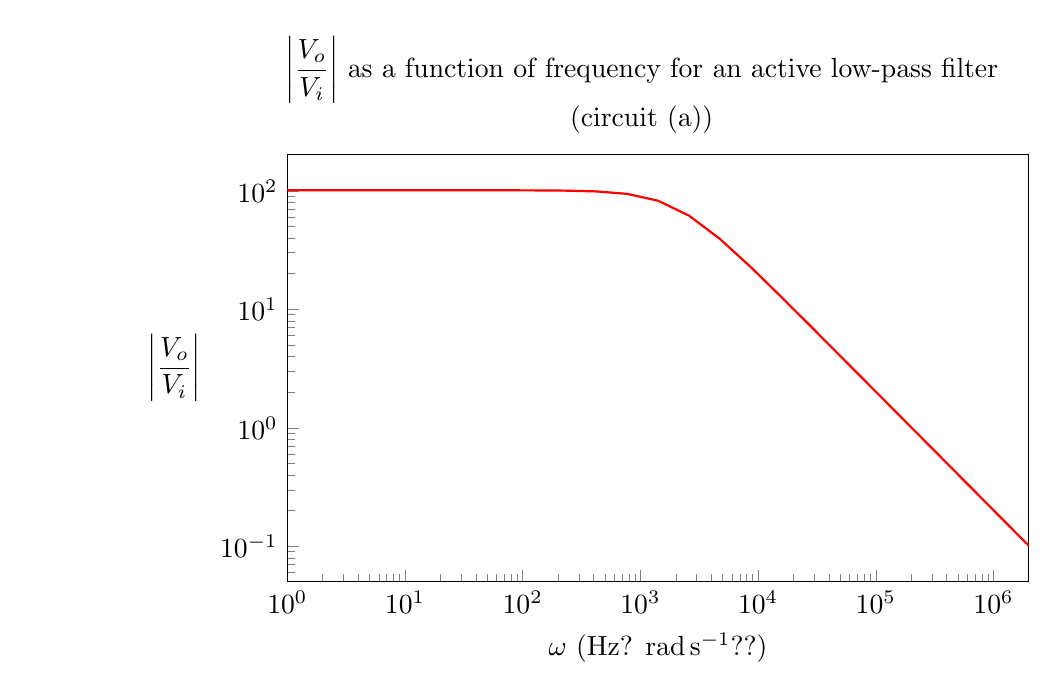
\begin{tikzpicture}[scale = 1]
              \begin{axis}[
                  xmode=log,
                  ymode=log,
                  xmin=1,
                  xmax=2000000,
                  ylabel style={rotate=-90},
                  xlabel={$\omega$ ($\unit{\hertz}$? $\unit{\radian\per\second}$??)},
                  ylabel={~~~~~~~~~~~~$\displaystyle\left|\frac{V_o}{V_i}\right|$}, % Gross.
                  xtick pos=bottom,
                  ytick pos=left,
                  width=11cm,
                  height=7cm
                ]
                \addplot[thick,red,domain=1:2000000] (\x,{(101*sqrt(1+(1000^(2))*(\x*500*10^(-9))^2))/(((\x*500*10^(-9))^(2))*((1000^2)+(\x*500*10^(-9))^(-2)))});
              \end{axis}
              \node[align=center] (title) at (4.5,6.3) {$\displaystyle\left|\frac{V_o}{V_i}\right|$ as a function of frequency for an active low-pass filter \\ (circuit (a))};
            \end{tikzpicture}

            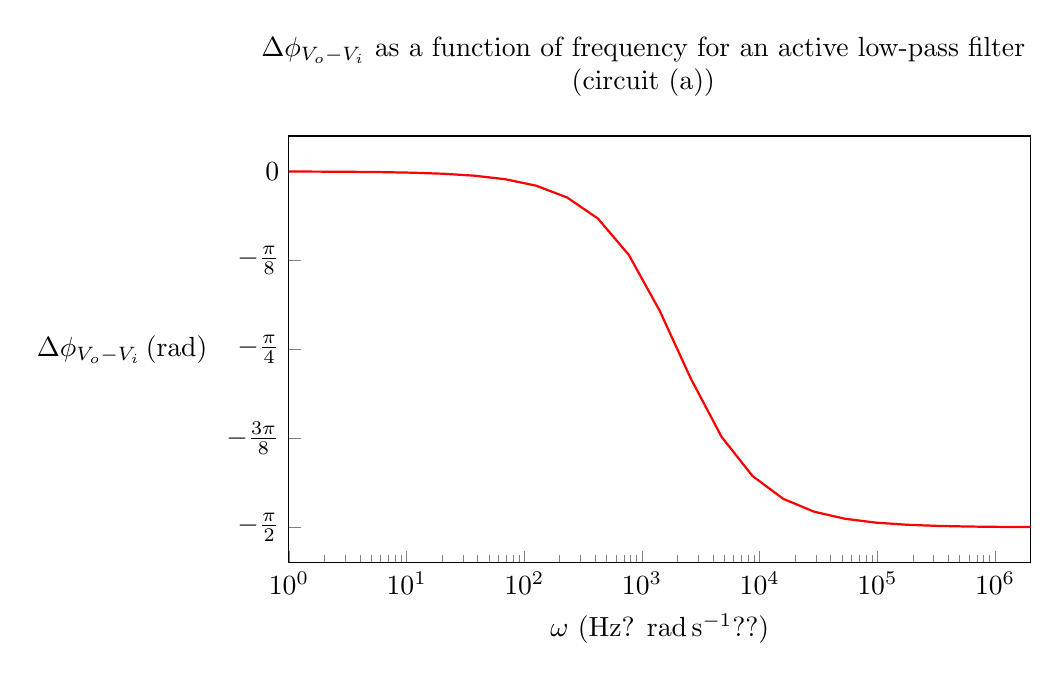
\begin{tikzpicture}
              \begin{axis}[
                  xmode=log,
                  xmin=1,
                  xmax=2000000,
                  ylabel style={rotate=-90},
                  xlabel={$\omega$ ($\unit{\hertz}$? $\unit{\radian\per\second}$??)},
                  ylabel={$\Delta\phi_{V_o-V_i}\, (\unit{\radian})$},
                  xtick pos=bottom,
                  ytick pos=left,
                  width=11cm,
                  height=7cm,
                  ytick={
                      0, -pi/8, -pi/4, (-3*pi)/8, -pi/2
                    },
                  yticklabels={
                      $0$, $-\frac{\pi}{8}$, $-\frac{\pi}{4}$, $-\frac{3\pi}{8}$, $-\frac{\pi}{2}$
                    }
                ]
                \addplot[thick,red,domain=1:2000000] (\x,{pi/180*atan(-1000*\x*500*10^(-9))});
              \end{axis}
              \node[align=center] (title) at (4.5,6.3) {$\Delta\phi_{V_o-V_i}$ as a function of frequency for an active low-pass filter \\ (circuit (a))};
            \end{tikzpicture}
          \end{center}

          \begin{center}
            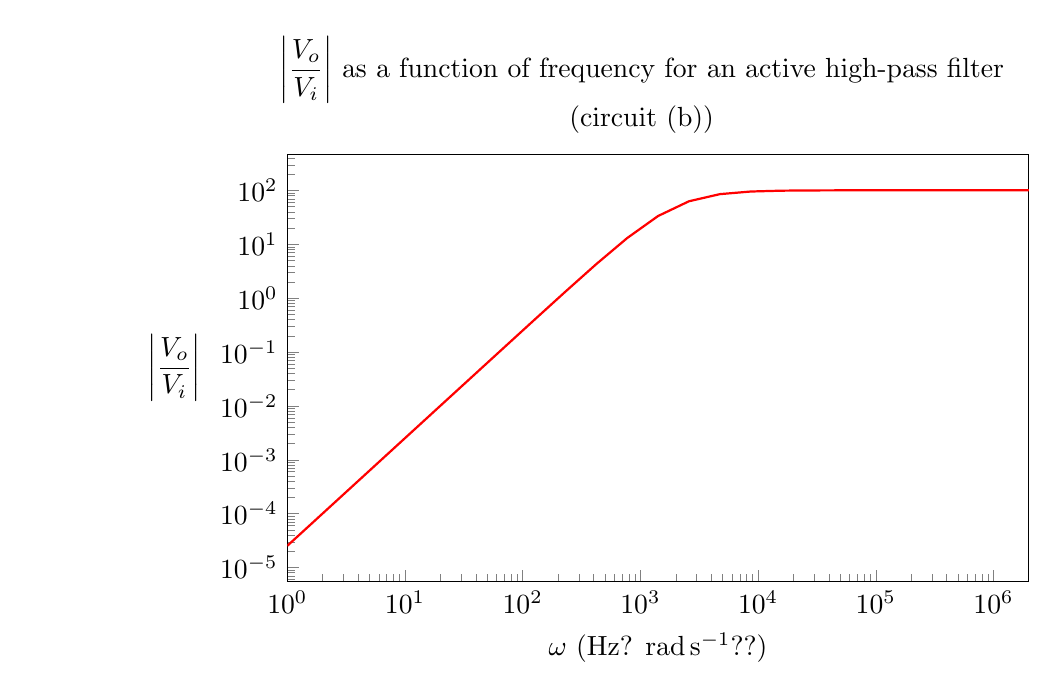
\begin{tikzpicture}[scale = 1]
              \begin{axis}[
                  xmode=log,
                  ymode=log,
                  xmin=1,
                  xmax=2000000,
                  ylabel style={rotate=-90},
                  xlabel={$\omega$ ($\unit{\hertz}$? $\unit{\radian\per\second}$??)},
                  ylabel={~~~~~~~~~~~~$\displaystyle\left|\frac{V_o}{V_i}\right|$}, % Gross.
                  xtick pos=bottom,
                  ytick pos=left,
                  width=11cm,
                  height=7cm
                ]
                \addplot[thick,red,domain=1:2000000] (\x,{(101*1000*sqrt(1+(1000^2)))/((1000^2)+(\x*500*10^(-9))^(-2))});
              \end{axis}
              \node[align=center] (title) at (4.5,6.3) {$\displaystyle\left|\frac{V_o}{V_i}\right|$ as a function of frequency for an active high-pass filter \\ (circuit (b))};
            \end{tikzpicture}

            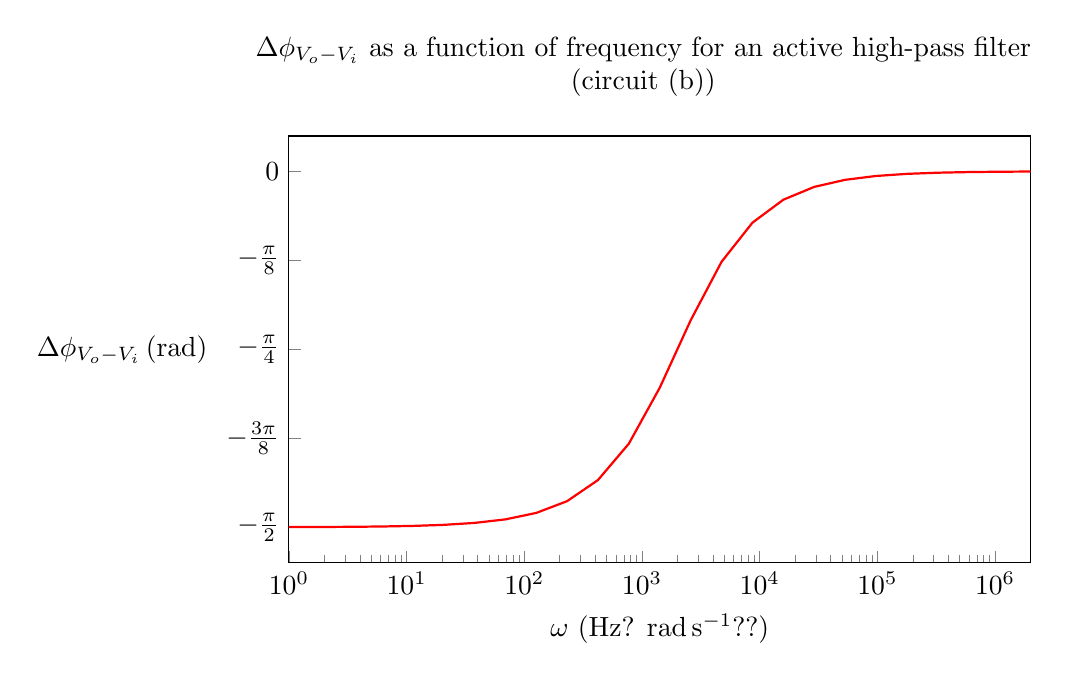
\begin{tikzpicture}
              \begin{axis}[
                  xmode=log,
                  xmin=1,
                  xmax=2000000,
                  ylabel style={rotate=-90},
                  xlabel={$\omega$ ($\unit{\hertz}$? $\unit{\radian\per\second}$??)},
                  ylabel={$\Delta\phi_{V_o-V_i}\, (\unit{\radian})$},
                  xtick pos=bottom,
                  ytick pos=left,
                  width=11cm,
                  height=7cm,
                  ytick={
                      0, -pi/8, -pi/4, (-3*pi)/8, -pi/2
                    },
                  yticklabels={
                      $0$, $-\frac{\pi}{8}$, $-\frac{\pi}{4}$, $-\frac{3\pi}{8}$, $-\frac{\pi}{2}$
                    }
                ]
                \addplot[thick,red,domain=1:2000000] (\x,{pi/180*atan((-1000*\x*500*10^(-9))^(-1))});
              \end{axis}
              \node[align=center] (title) at (4.5,6.3) {$\Delta\phi_{V_o-V_i}$ as a function of frequency for an active high-pass filter \\ (circuit (b))};
            \end{tikzpicture}
          \end{center}
    \item For circuit (a)
          \begin{align*}
             & 1=\frac{101\sqrt{1+R^2(\omega C)^2}}{(\omega C)^2\left(R^2+(\omega C)^{-2}\right)} \\
             & (\omega C)^2R^2+1=101\sqrt{1+R^2(\omega C)^2}                                      \\
             & \frac{(\omega C)^2R^2+1}{\sqrt{1+R^2(\omega C)^2} }=101                            \\
             & \omega=\sqrt{\frac{101^2-1}{(RC)^2}}=201990whatevertheunitofthegraphaboveis
          \end{align*}
          For circuit (b)
          \begin{align*}
             & 1=\frac{101R\sqrt{1+R^2}}{R^2+(\omega C)^{-2}}      \\
             & R^2+(\omega C)^{-2}=101R\sqrt{1+R^2}                \\
             & \omega=\sqrt{\frac{1}{101RC^2\sqrt{1+R^2}-(RC)^2}}\approx200 \\
          \end{align*}
  \end{enumerate}
\end{soln}
\end{document}